% Chapter Template

\chapter{Ensayos y resultados} % Main chapter title

\label{Chapter4} % Change X to a consecutive number; for referencing this chapter elsewhere, use \ref{ChapterX}

%----------------------------------------------------------------------------------------
%	SECTION 1
%----------------------------------------------------------------------------------------

\section{Pruebas funcionales de hardware}
%\label{sec:pruebasHW}

En el presente capítulo se explican los ensayos realizados sobre el prototipo del equipo dip coater, se presentan y analizan los resultados obtenidos y se introducen posibles cambios para próximas versiones.
\subsection{Comunicación con driver TMC5130}

El presente ensayo se realizó para verificar la comunicación entre el microcontrolador ESP32 y el CI TMC5130. Como se mencionó en el capítulo \ref{Chapter3} dicha comunicación se establece a través del  protocolo SPI. En la figura \ref{fig:ensayo_spi_0} se observa el esquema del banco de pruebas propuesto.

\begin{figure}[h]
\centering 
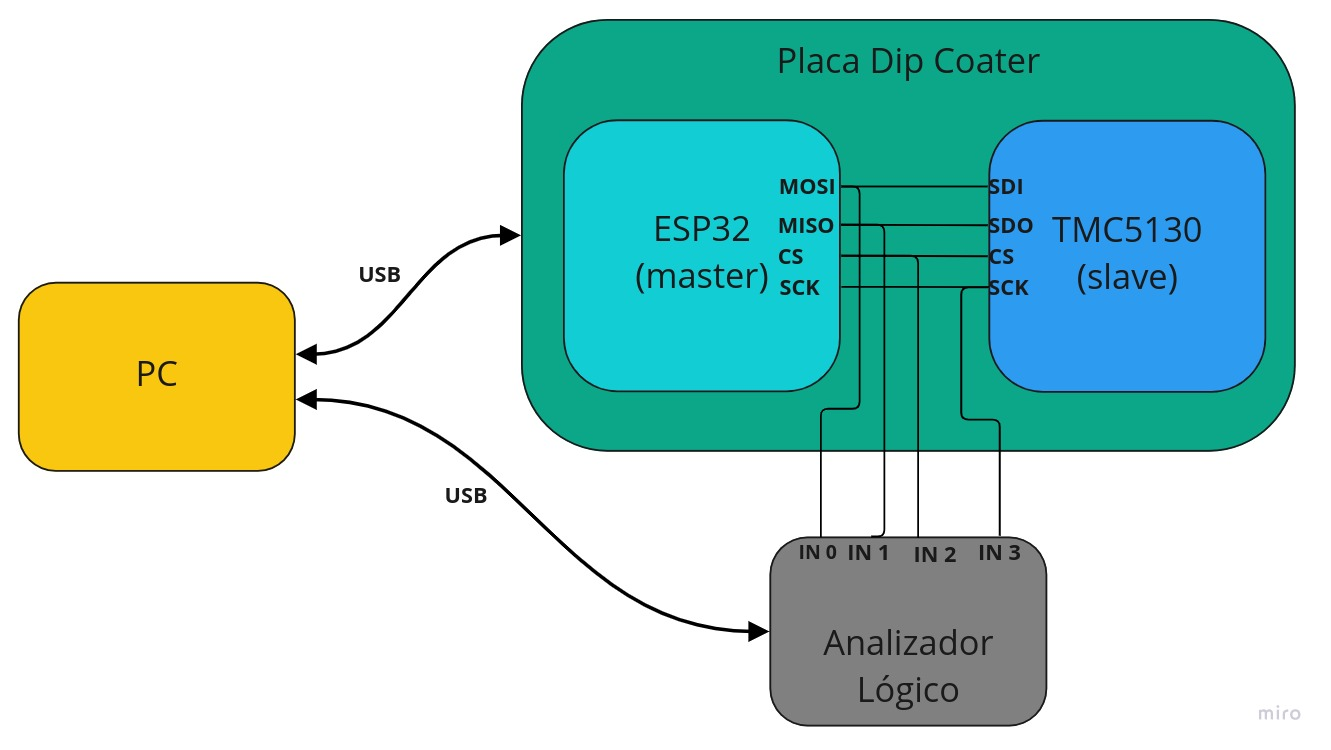
\includegraphics[width=1\textwidth]{./Figures/ensayo_spi.jpg}
\caption{Banco de pruebas.}
\label{fig:ensayo_spi_0}
\end{figure}


 
% Al encender el equipo se realiza una configuración inicial en donde se escriben todos los registros y luego durante el uso del equipo se realizan operaciones de lectura y escritura para conocer el estado del CI y accionar diferentes tipos de movimientos.
%Se configura el ESP como dispositivo \textit{SPI master} y el TMC5130 como dispositivo \textit{SPI slave}.

%En la figura \ref{fig:datagrama} se observa la estructura de datos para leer y escribir registros.
%\begin{figure}[h]
%\centering 
%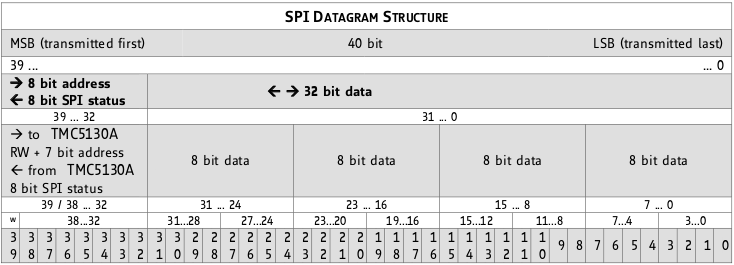
\includegraphics[width=1\textwidth]{./Figures/datagrama.png}
%\caption{Datagrama de 40 bits.}
%\label{fig:datagrama}
%\end{figure}


%Las operaciones de lectura y escritura tienen una diferencia, que se ve representada por el bit más significativo de la trama de datos, es decir el bit 39. Cuando la operación es de lectura, y primer byte que representa la dirección del registro no sufre alteración. Cuando la operación es de escritura, se debe establecer en 1 el bit de la posición 39. Por ejemplo, si  se pretende escribir un valor en el registro [0x22], el primer byte del datagrama deberá ser [0x22 + 0x80 = 0xA2],  sumar [0x80] representa poner en 1 el primer bit del byte mas significativo del datagrama. 


Para realizar el ensayo se conectó de manera provisoria el analizador lógico USB con las cuatro terminales que establecen la comunicación SPI entre el microcontrolador y el CI TMC5130. La comunicación con el CI TMC5130 está definida por datagramas de 5 bytes, el primer byte define la dirección del registro y los 4 bytes restantes representan su valor. Las operaciones de lectura y escritura tienen una diferencia que se representa en el byte de dirección. Cuando la operación es de escritura, se debe establece en 1 el bit mas significativo de dicho byte y cuando la operación es de lectura, la dirección no sufre alteración.

Se puede observar en la figura \ref{fig:ensayo_spi} el banco de pruebas.

\begin{figure}[h]
\centering 
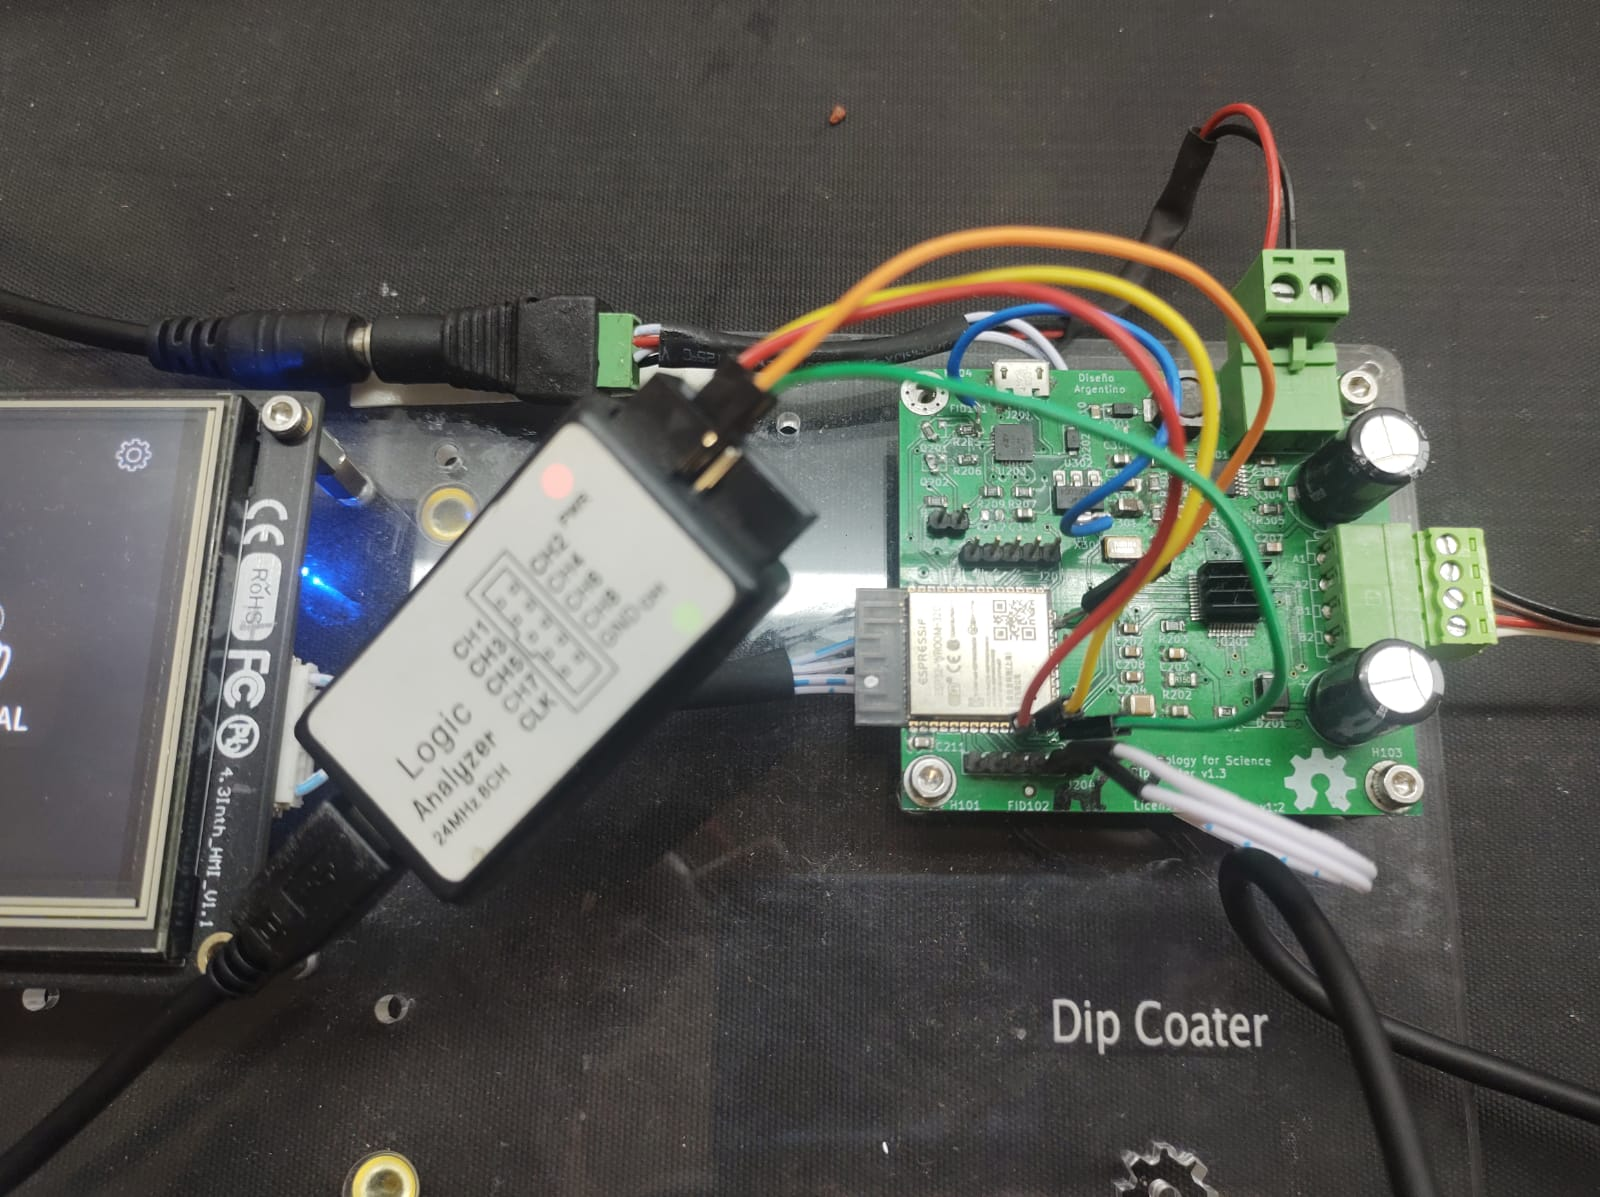
\includegraphics[width=0.8\textwidth]{./Figures/ensayo_spi.jpeg}
\caption{Ensayo sobre terminales SPI.}
\label{fig:ensayo_spi}
\end{figure}

El procedimiento realizado fue el siguiente:
\begin{enumerate}
\item Se conectó el equipo dip coater con el software Putty para establecer una consola de comandos.
\item Se ejecutó el software del analizador lógico y se comenzó el registro de datos.
\item Se ejecutó el comando de lectura del registro [0x2D].
\item Se ejecutó el comando de escritura del registro [0x2D] con valor [0x00 0XFF 0x00 0x00].
\item Se realizó nuevamente una lectura del registro [0x2D] para verificar el valor ingresado en el item anterior. 
\end{enumerate}


En la figura \ref{fig:ensayo_spi_a} se observa la ejecución del comando de lectura sobre el registro [0x2D]. 
\begin{itemize}
\item MOSI: [0x2D][0x00 0x00 0x00 0x00].
\item MISO: [0x29][0x00 0x01 0xF8 0x88].
\end{itemize}



\begin{figure}[h]
\centering 
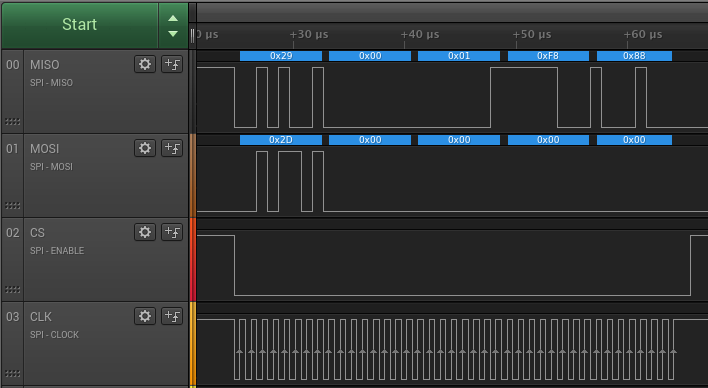
\includegraphics[width=1\textwidth]{./Figures/ensayo_spi_a.png}
\caption{Comando de lectura sobre registro [0x2D].}
\label{fig:ensayo_spi_a}
\end{figure}


En la figura \ref{fig:ensayo_spi_b} se observa la ejecución del comando de escritura sobre el registro [0x2D] con valor [0x00 0xFF 0xFF 0x00]. 

\begin{itemize}
\item MOSI: [0x2D + 0x80 = 0xAD][0x00 0xFF 0x00 0x00].
\item MISO: [0x11][0x00 0x01 0xF8 0x88].
\end{itemize}



\begin{figure}[h]
\centering 
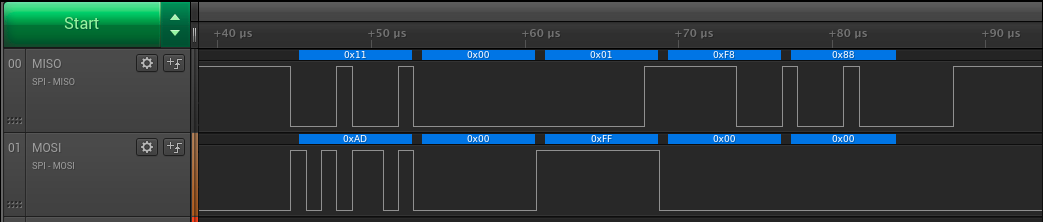
\includegraphics[width=1\textwidth]{./Figures/ensayo_spi_b.png}
\caption{Comando de escritura sobre registro [0x2D].}
\label{fig:ensayo_spi_b}
\end{figure}

En la figura \ref{fig:ensayo_spi_c} se observa la ejecución nuevamente del comando de lectura sobre el registro [0x2D].

\begin{itemize}
\item MOSI: [0x2D][0x00 0xFF 0x00 0x00].
\item MISO: [0x11][0x00 0xFF 0x00 0x00].
\end{itemize}


\begin{figure}[h!]
\centering 
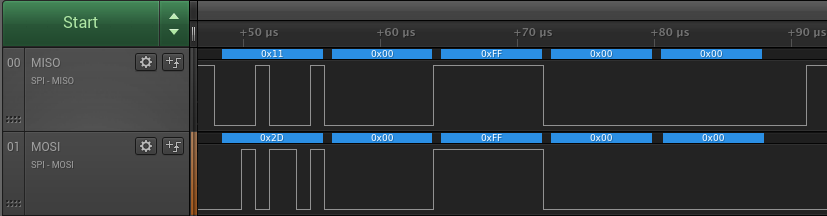
\includegraphics[width=1\textwidth]{./Figures/ensayo_spi_c_c.png}
\caption{Comando de lectura actualizado sobre registro [0x2D].}
\label{fig:ensayo_spi_c}
\end{figure}

Se observa entonces que luego de estas operaciones el registro [0x2D] se actualizó correctamente con el valor[0x00 0xFF 0x00 0x00].

Con este ensayo se validó la comunicación SPI entre el microcontrolador y el CI TMC5130 para las operaciones de lectura y escritura de datos.

%\subsection{Comunicación con pantalla táctil}
%El presente ensayo se realizó para verificar la comunicación entre el microcontrolador ESP32 y la pantalla táctil STONE . Como se mencionó en el capítulo \ref{Chapter3} dicha comunicación se establece a través del  protocolo serial.
%El banco de pruebas fue el siguiente:



\section{Pruebas funcionales del firmware}
\subsection{Tiempo de ejecución de movimientos}

El ensayo se realizó para verificar los parámetros que definen el desplazamiento de la muestra, es decir para verificar que las velocidades y aceleraciones que definen movimientos sean similares a las que surgen del cálculo teórico.

En el capítulo \ref{Chapter3} se detalló la configuración de la rampa de cuatro puntos que define los movimientos del equipo. 
%Puntos que define un movimiento y se mostró la configuración de los parámetros para obtener una rampa de cuatro puntos en donde la etapa de aceleración es igual a la etapa de desaceleración.

Dicha rampa está definida por la ecuación \ref{eq:movimiento_completo}.

\begin{equation}
	\label{eq:movimiento_completo}
	\vec{x}=\vec{x_o}+\vec{v}(t-t_o)+\frac12 \vec {a} (t-t_o)^2
\end{equation}
%(((2*velocidad)/(aceleración*1000))+(desplazamiento/velocidad))*60*1000  

Por lo tanto, con los valores de aceleración, desaceleración, velocidad y desplazamiento se calculó el tiempo teórico necesario para la ejecución de un movimiento.
En la tabla \ref{tab:ensayo_comandos} se observan los valores de los parámetros ensayados.

\begin{table}[h]
	\centering
	\caption[Ensayo de tiempo en desplazamientos]{Ensayo de tiempos en desplazamiento}
	\begin{tabular}{c c c }    
		\toprule
		\textbf{Velocidad (mm/min)}     & \textbf{Aceleración-Desaceleración(m/min)} & \textbf{Desplazamiento(mm)} \\
		\midrule
		1  mm/min	 & 	   100-500-1000-2100 m/min2     & 	50 mm 			 	\\		
		10  mm/min   & 	   100-500-1000-2100 m/min2 	& 	50 mm				\\
		100  mm/min  & 	   100-500-1000-2100 m/min2	    & 	50 mm 				\\
		200  mm/min	 & 	   100-500-1000-2100 m/min2	    & 	50 mm 			\\
		500  mm/min	 & 	   100-500-1000-2100 m/min2     & 	50 mm					\\
		800  mm/min	 & 	   100-500-1000-2100 m/min2     & 	50 mm					\\
		\bottomrule
		\hline
	\end{tabular}
	\label{tab:ensayo_comandos}
\end{table}

Para realizar el ensayo se implementó una aplicación de prueba que realiza el siguiente procedimiento:

\begin{enumerate}
\item Configuración de movimiento descendente con valores de velocidad, aceleración y desplazamiento.
\item Ejecución del movimiento descendente y registro del tiempo del sistema.
\item Registro del tiempo del sistema al final del movimiento, cálculo de variación temporal y envío del dato por terminal serie.
\item Configuración y ejecución de movimiento ascendente con valores de velocidad, aceleración y desplazamiento.
\item Ejecución del movimiento ascendente y registro del tiempo del sistema.
\item Registro del tiempo del sistema al final del movimiento, cálculo de variación temporal y envío del dato por terminal serie.
\item Incremento de la tabla hacia nuevos parámetros de aceleración, velocidad y desplazamiento.
\item Repetición del ciclo.
\end{enumerate}

Un ordenador conectado al equipo ejecuta un script de Python que guarda los datos recibidos en un archivo.

En la figura \ref{fig:tiempo_movimiento_1} se observa una comparación de tiempos teóricos respecto a  tiempos registrados en el sistema. En el eje Y se representa el tiempo en milisegundos necesario para ejecutar cada movimiento y en el eje X la velocidad. Los puntos cercanos representan el movimiento descendente y ascendente con el mismos parámetro de velocidad y aceleración, por tal motivo se visualizan pares de puntos cercanos. El gráfico compara los tiempos teórico respecto a los tiempos registrados. A simple vista no se pueden visualizar diferencias significativas.

\begin{figure}[h]
\centering 
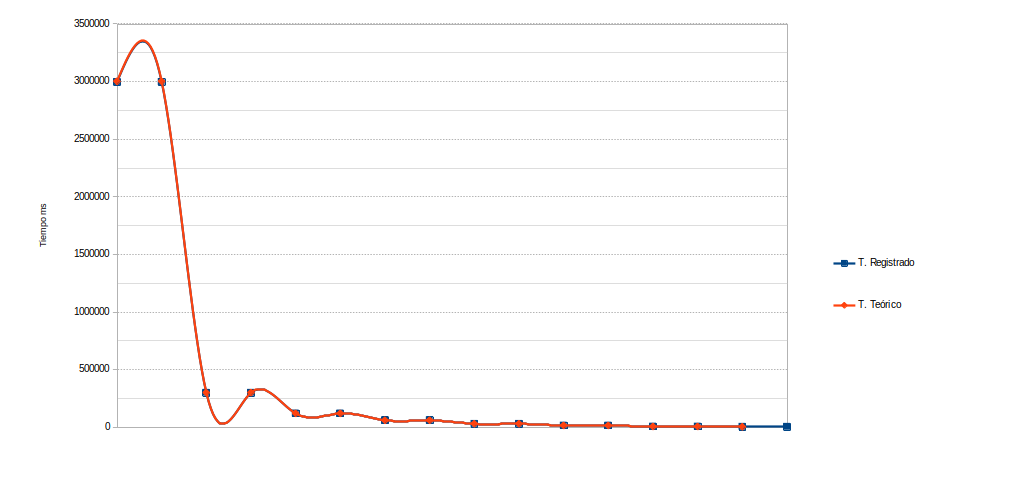
\includegraphics[width=1\textwidth]{./Figures/tiempo_movimiento_1.png}
\caption{Comparación de tiempos teóricos y registrados.}
\label{fig:tiempo_movimiento_1}
\end{figure}

Se presenta en la figura \ref{fig:error_porcentual_1} un gráfico que representa los errores relativos porcentuales de las mediciones realizadas. Se puede observar que existe un aumento del error relativo a velocidades altas, con un registro pico  en la velocidad de 800 mm/min. 


\begin{figure}[h]
\centering 
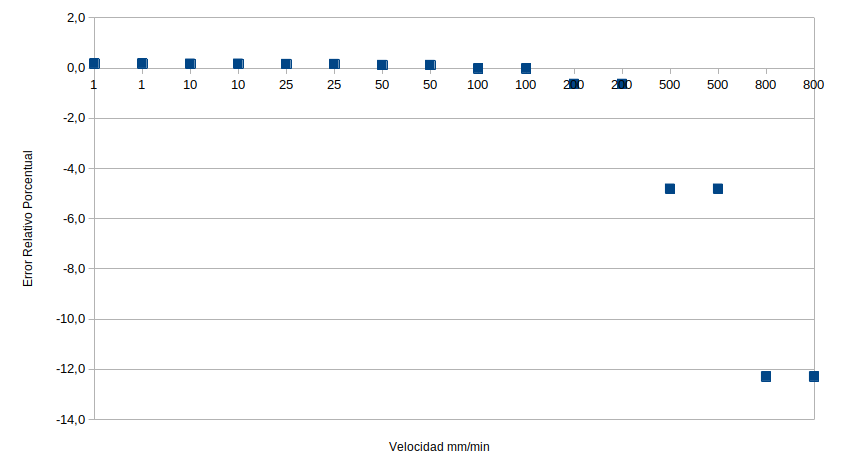
\includegraphics[width=1\textwidth]{./Figures/error.png}
\caption{Error relativo porcentual.}
\label{fig:error_porcentual_1}
\end{figure}
Se concluye con este ensayo que el equipo es muy preciso en la mayor parte del rango para el cual fue diseñado teniendo un error relativo pico de 13\% en las velocidades superiores del rango de funcionamiento.
 
  
\section{Calibración del equipo}
\label{sec:calibración}
\subsection{Desplazamiento lineal y micro pasos}

Este ensayo se realizó para definir y ajustar la constante de desplazamiento que relaciona los micro pasos realizados por el motor, con la distancia de desplazamiento del carro. La misma es una constante que está definida por el paso del tornillo sobre el cual se desplaza el carro.

Para realizar las mediciones se utilizó un comparador digital de la marca Asimeto\citep{web_asimeto}, el cual puede observarse en la figura \ref{fig:micrometro}. El mismo tiene una resolución de 0.001 mm y permite desplazamientos de 0 a 50 mm.


\begin{figure}[h]
\centering 
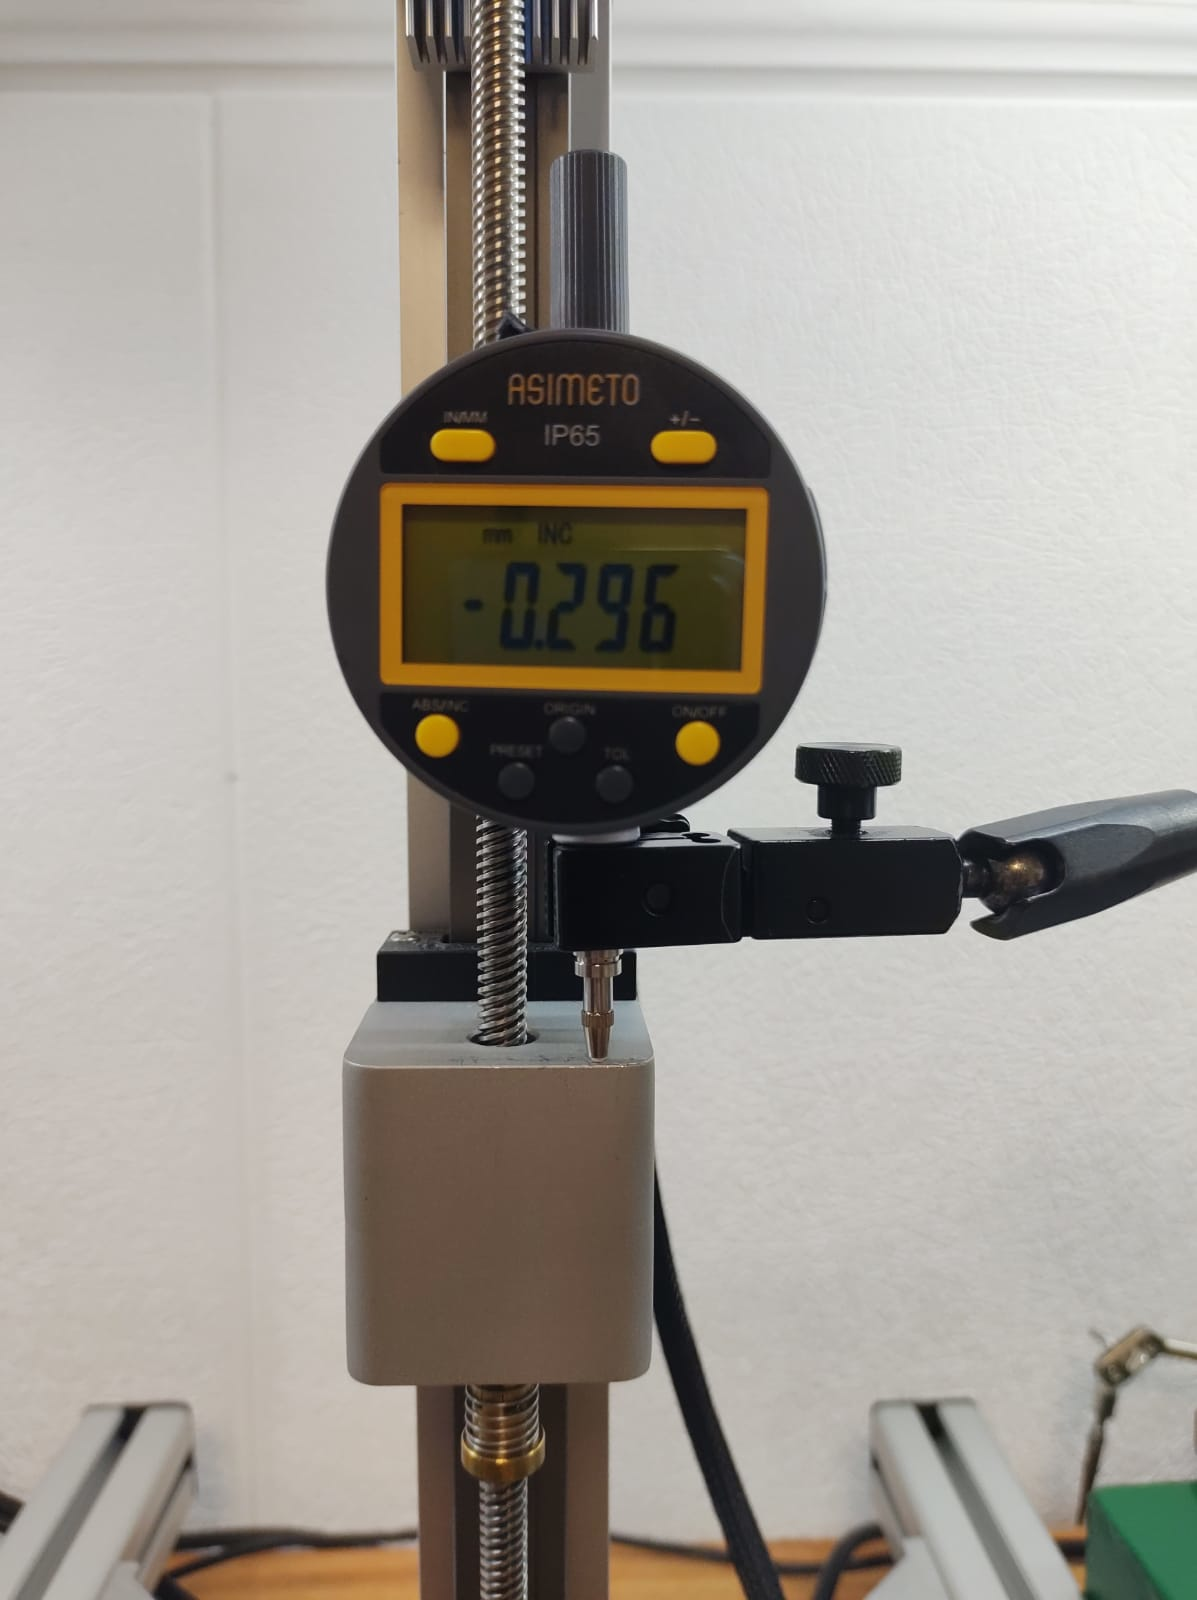
\includegraphics[width=0.3\textwidth]{./Figures/micrometro.png}
\caption{Comparador digital Asimeto.}
\label{fig:micrometro}
\end{figure}

El ensayo consistió en medir seis desplazamientos sucesivos de 1 mm sobre el carro de manera descendente y luego de manera ascendente. Este ensayo es importante porque permite corregir la unidad de conversión de micro pasos a milímetros que utiliza el CI TMC5130 para realizar todos los movimientos. 
En la subsección \ref{subsec:calibracion} se mencionó la macro \textit{MACHINE STEPS PER MILLIMETER} definida en el archivo hardware.h que surgió de este ensayo. 

En la figura \ref{fig:desplazamiento_lineal} se observa el banco de medición donde se visualiza el comparador Asimeto apoyado sobre una base metálica independiente, con la punta del mismo en contacto directo con el carro de desplazamiento.

\begin{figure}[h]
\centering 
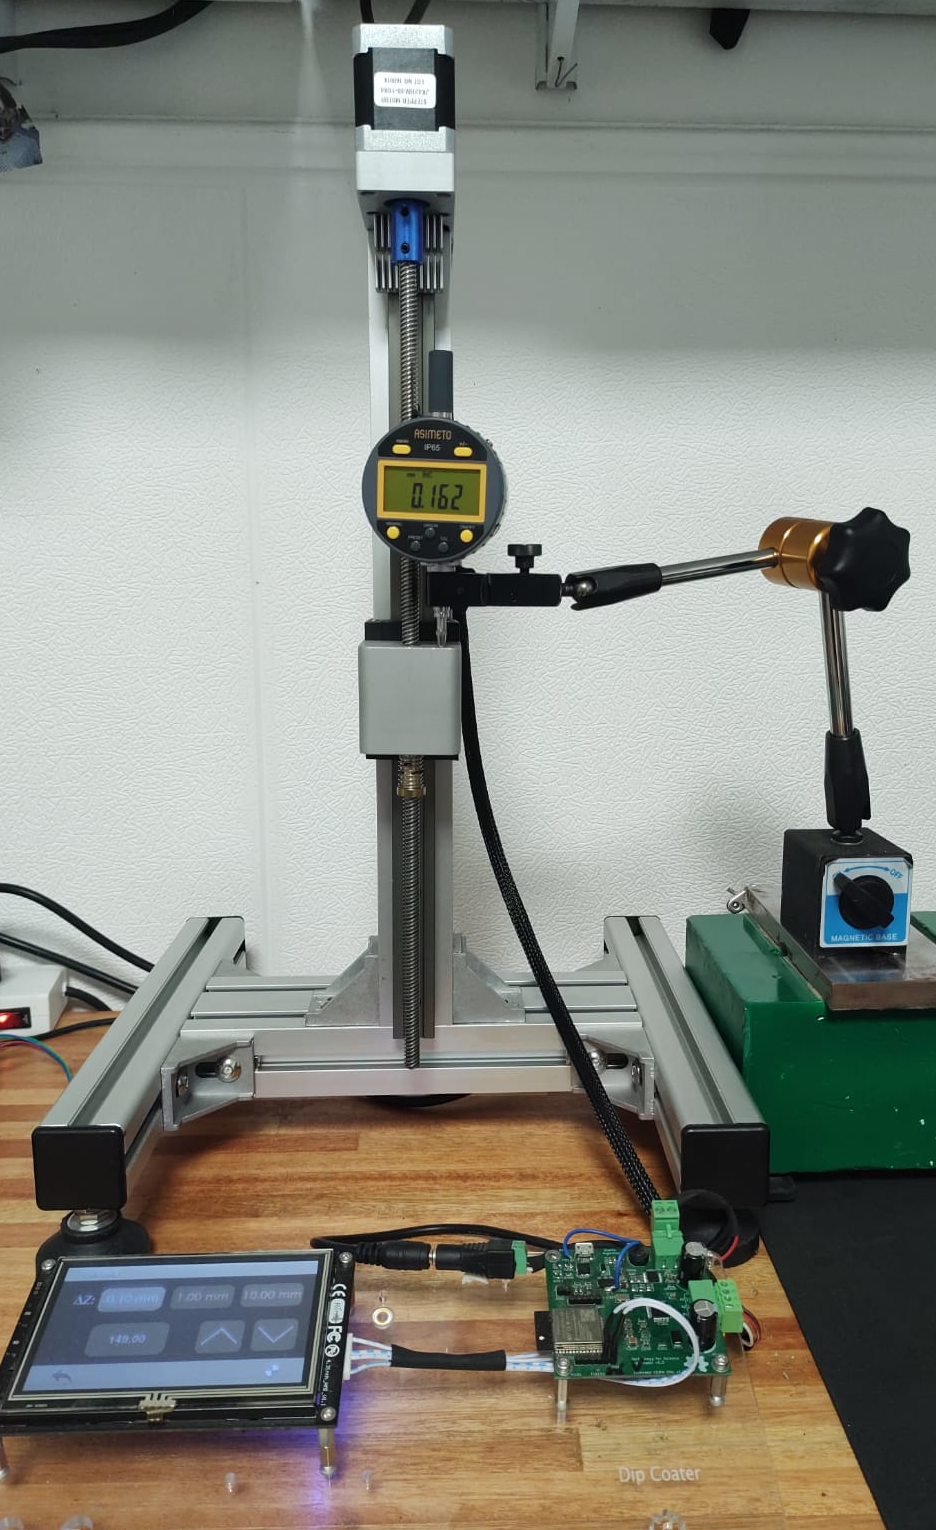
\includegraphics[width=0.5\textwidth]{./Figures/desplazamiento_lineal.png}
\caption{Ensayo de desplazamiento lineal.}
\label{fig:desplazamiento_lineal}
\end{figure}


Para iniciar el ensayo se presiona el botón \textit{origin} del comparador para poner en cero la medida, la sensibilidad del mismo es tan grande que es difícil lograr 0,000 mm debido a la acción misma  de apretar el botón. Luego se realizan movimientos descendentes de 1 mm y se registran los datos.
En la tabla \ref{tab:ensayo_desplazamiento_des} se muestran los resultados obtenidos.

\begin{table}[h!]
	\centering
	\caption[Ensayo de desplazamiento]{Ensayo de desplazamiento lineal descendente}
	\begin{tabular}{l c c }    
		\toprule
		\textbf{Posición absoluta}     & \textbf{Desplazamiento} & \textbf{Error Relativo} \\
		\midrule
		0,058 mm	& 	        	& 	 			 	\\		
		1,051 mm    & 	0,993 mm    	& 	0,007				\\
		2,035 mm 	& 	0,984 mm	    & 	0,016 				\\
		3,034 mm	& 	0,999 mm	    & 	0,001 			\\
		4,054 mm 	& 	1,02 mm         & 	-0,020					\\
		5,039 mm 	& 	0,985 mm	    & 	0,015					\\
		5,998 mm 	& 	0,959 mm        & 	0,041 			\\
		\bottomrule
		\hline
	\end{tabular}
	\label{tab:ensayo_desplazamiento_des}
\end{table}

De igual manera se confecciona la tabla \ref{tab:ensayo_desplazamiento_asc} para los movimientos ascendentes.
 
\begin{table}[h!]
	\centering
	\caption[Ensayo de desplazamiento]{Ensayo de desplazamiento lineal ascendente}
	\begin{tabular}{l c c }    
		\toprule
		\textbf{Posición absoluta}     & \textbf{Desplazamiento} & \textbf{Error Relativo} \\
		\midrule
		0,02 mm	& 	        	& 	 			 	\\		
		0,939 mm    & 	0,019 mm    	& 	0,081	\\
		1,931 mm 	& 	0,992 mm	    & 	0,008 	\\
		2,929 mm	& 	0,998 mm	    & 	0,002 	\\
		3,923 mm 	& 	0.994 mm        & 	0,006	\\
		4,923 mm 	& 	1 mm	    	& 	0		\\
		5,911 mm 	& 	0,988 mm        & 	0,012 	\\
		\bottomrule
		\hline
	\end{tabular}
	\label{tab:ensayo_desplazamiento_asc}
\end{table}


Para corregir el valor de micro pasos por milímetros de desplazamiento se utilizó el siguiente procedimiento:
\begin{enumerate}
\item Realizar un promedio de los 6 errores relativos ascendentes y descendentes.
\item Ajustar el valor inicial de micro pasos con los respectivos errores. 
\item Realizar un promedio entre el valor corregido ascendente y el valor corregido descendente.
\end{enumerate}


Inicialmente al comenzar el ensayo la macro \textit{MACHINE STEPS PER MILLIMETER}  estaba definida con un valor de 12737 micro pasos por milímetros, luego de sucesivas correcciones la macro quedo definida en 12932 micro pasos por milímetros.
Este ensayo se repitió cinco veces hasta llegar a los valores presentados en las tablas anteriores, en donde se observó que el porcentaje promedio de los errores relativos fue inferior al 2.5\%.

\section{Caso de prueba}
\section{Prueba de campo con personal capacitado}

El siguiente ensayo consistió en una prueba completa del equipo dip coater con personal capacitado del Instituto de Nanosistemas.
La prueba que se llevo a cabo consistió en realizar el primer \textit{thin films} del equipo, se utilizó un wafer de silicio como sustrato y una solución de dioxido de titanio disuelto en etanol para formar un film de nanoparticulas de titanio.

\begin{figure}[h]
\centering 
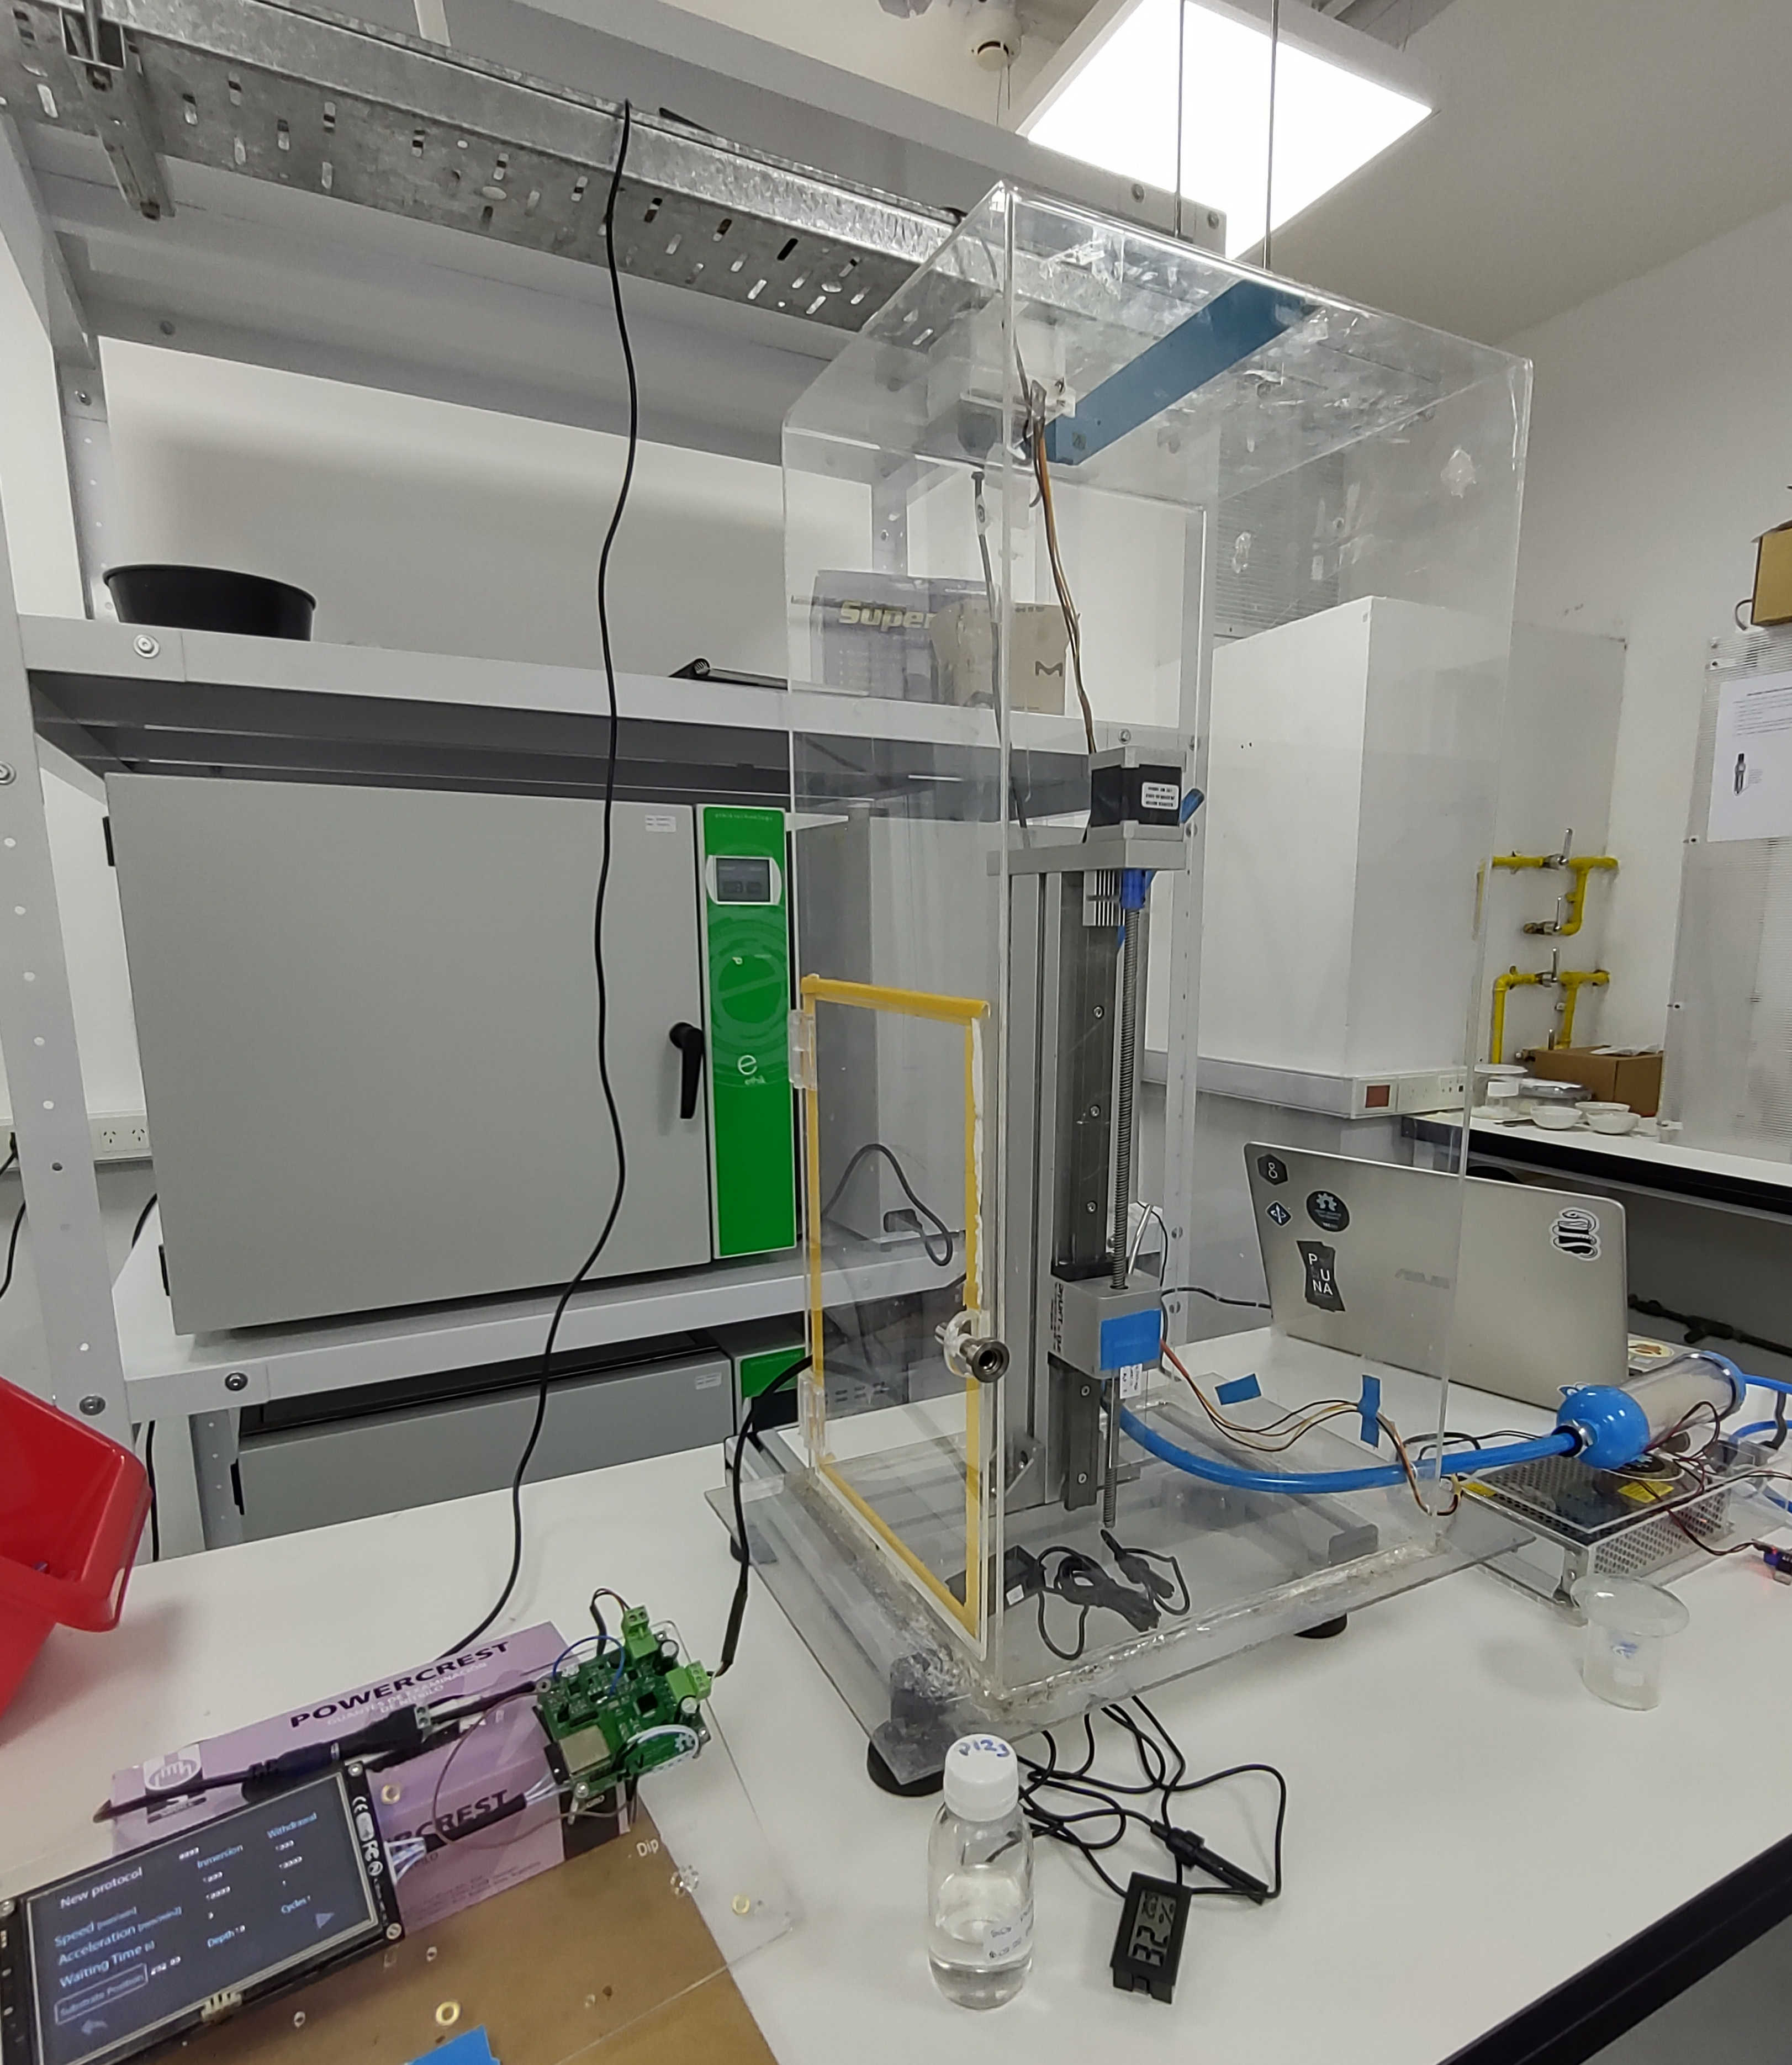
\includegraphics[width=0.5\textwidth]{./Figures/prueba_b.jpg}
\caption{Ensayo completo en laboratorio.}
\label{fig:desplazamiento_lineal}
\end{figure}


\begin{figure}[h]
\centering 
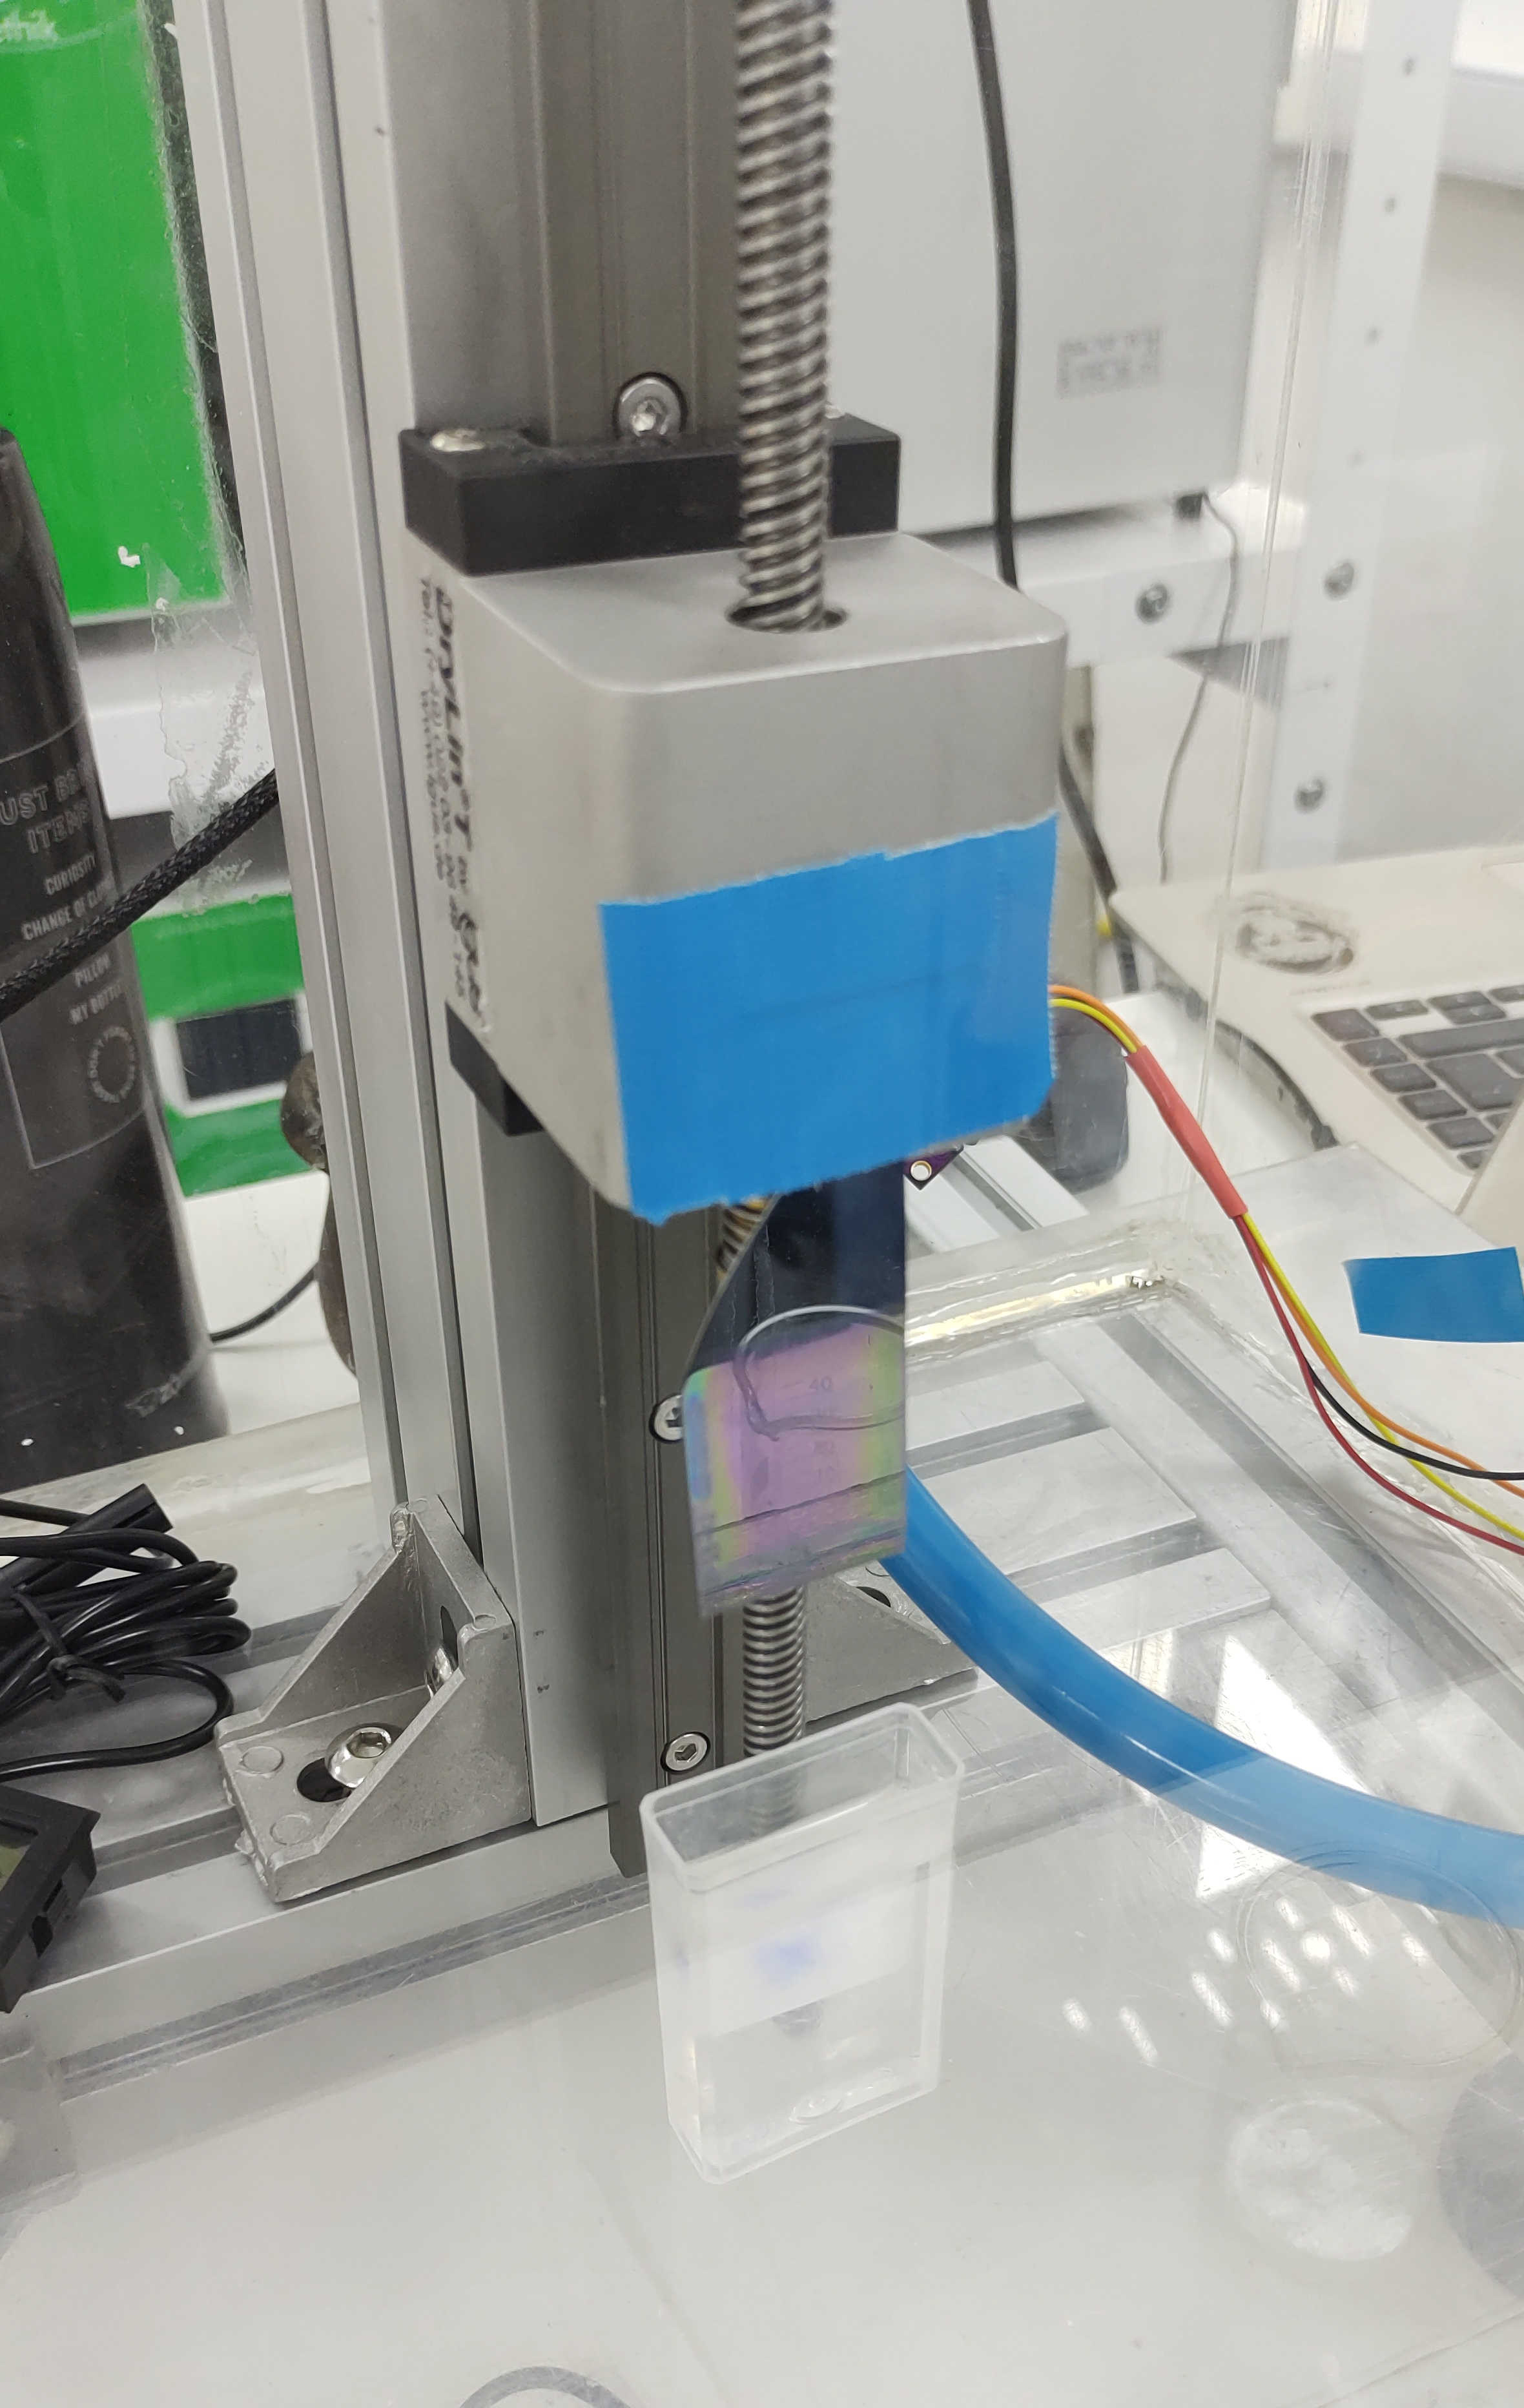
\includegraphics[width=0.5\textwidth]{./Figures/prueba_a.jpg}
\caption{Ensayo con wafer de silicio.}
\label{fig:desplazamiento_lineal}
\end{figure}


